\documentclass[dvipdfmx]{jsarticle}
\usepackage{tikz}
\usetikzlibrary{arrows}
\usetikzlibrary{intersections, calc}
\begin{document}
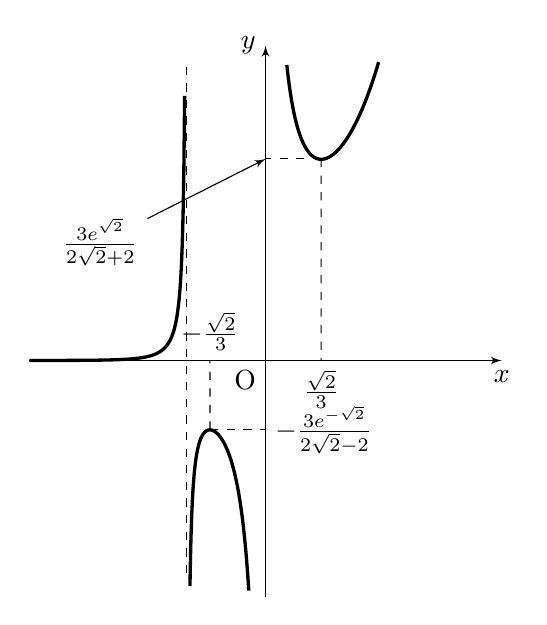
\begin{tikzpicture}[xscale = 1.5,yscale = 1, >=latex']

% axis
\node(O) at (0,0) [below left]{$\mathrm{O}$};
\draw[->] (-2,0) -- (2,0) node[below]{$x$};
\draw[->] (0,-3) -- (0,4) node[left]{$y$};

% coordinates
\draw[dashed] ( -0.47, - 0.88) --  ( - 0.471,0) node[above]{$ - \frac{\sqrt{2} }{3}$};
\draw[dashed] ( -0.47, - 0.88) --  ( 0, -0.88) node[right]{$- \frac { 3 e ^ { - \sqrt { 2 } } } { 2 \sqrt { 2 } - 2 }$};
\draw[dashed] ( 0.47, 2.56) --  (  0.471,0) node[below]{$ \frac{\sqrt{2} }{3}$};
\coordinate(N) at (0, 2.56);
\draw[dashed] ( 0.47, 2.56) --  (N);
\node(M) at ( - 1,1.5) [left] {$\frac { 3 e ^ { \sqrt { 2 } } } { 2 \sqrt { 2 } + 2 }$};
\draw[->,thin] (M) -- (N);
\draw[dashed] ( - 0.67, -2.7) -- ( - 0.67,3.8);

% curve
\draw [very thick, domain=-2.0:-0.682177, samples=200] plot(\x, {exp(3*\x) / (\x * (3*\x + 2))});
\draw [very thick, domain=-0.64:-0.14, samples=200] plot(\x, {exp(3*\x) / (\x * (3*\x + 2))});
\draw [very thick, domain=0.18:0.96, samples=200] plot(\x, {exp(3*\x) / (\x * (3*\x + 2))});

\end{tikzpicture}
\end{document}